\documentclass[apj]{emulateapj}

%Specify packages
\usepackage{amsmath}
\usepackage{tikz}
\usetikzlibrary{shapes.geometric, arrows}
\usepackage[tight]{subfigure}
\usepackage[breaklinks,colorlinks,citecolor=blue]{hyperref}
\usepackage[all]{hypcap}
\usepackage[utf8]{inputenc} %force unicode in bibtex
\usepackage{enumitem}
%use for editing/highlighting
\usepackage{color,soul}
%\usepackage{lineno}


%Define new commands as needed
\newcommand{\ang}{\AA~}
\defcitealias{barnes_inference_2016}{Paper I}
\renewcommand{\sectionautorefname}{Section}
\renewcommand{\subsectionautorefname}{Subsection}
%\linenumbers
%Set options for list spacing
\setenumerate{noitemsep}
%Set tikz options
\tikzstyle{box} = [rectangle, rounded corners, text centered, draw=black]
\tikzstyle{ghost} = [rectangle, rounded corners, text centered, draw=white]
\tikzstyle{arrow} = [thick, ->, >=stealth]

\begin{document}
	%Frontmatter
	\title{Inference of Heating Properties from ``Hot'' Non-flaring Plasmas in Active Region Cores II. Nanoflare Trains}
	\shorttitle{``Hot'' Non-flaring Plasmas II. Nanoflare Trains}
	\author{W. T. Barnes}
	\affil{Department of Physics \& Astronomy, Rice University, Houston, TX 77251-1892}
	\email{will.t.barnes@rice.edu}
	\author{P. J. Cargill}
	\affil{Space and Atmospheric Physics, The Blackett Laboratory, Imperial College, London SW7 2BW}
	\affil{School of Mathematics and Statistics, University of St. Andrews, St. Andrews, Scotland KY16 9SS}
	\and
	\author{S. J. Bradshaw}
	\affil{Department of Physics \& Astronomy, Rice University, Houston, TX 77251-1892}
	%Abstract
	\begin{abstract}
		Faint, high-temperature emission in active region cores has long been predicted as a signature of nanoflare heating. However, the detection of such emission has proved difficult due to a combination of the efficiency of thermal conduction, non-equilibrium ionization, and inadequate instrument sensitivity. In this second paper in our series on ``hot'' non-flaring plasma in active regions, we investigate the influence of repeating nanoflares of varying frequency on the resulting emission measure distribution . We have used an efficient two-fluid hydrodynamic model to carry out a parameter exploration in preferentially heated species, heating event frequency, and the power-law index determining the distribution of event energies. We compute the emission measure distribution for each point in our multi-dimensional heating parameter space in an effort to understand how each of these variables impacts the observed emission. Additionally, we calculate several observables and compare their efficacy in capturing the character of both the hot and cool parts of the emission measure distribution. 
	\end{abstract}
	%Body
	\section{Introduction}
	\label{sec:intro}
	%
	\par Heating of the solar corona by nanoflares, first proposed by \citet{parker_nanoflares_1988}, has become one of the most favored and contentious coronal heating models  \citep{cargill_implications_1994,cargill_nanoflare_2004,klimchuk_solving_2006}. The term \textit{nanoflare} has now become synonomous with impulsive heating in the energy range $10^{24}-10^{27}$ erg, with no specific assumption regarding the underlying physical mechanism; though its origin is almost certainly magnetic.
	%
	\par \citet{cargill_implications_1994,cargill_nanoflare_2004} have predicted that emission measure distributions resulting from nanoflare models should be wide and have a faint, high-temperature (8-10 MK) component, the so-called ``smoking gun'' of nanoflare heating. Though many workers \citep{reale_evidence_2009,schmelz_hinode_2009,miceli_x-ray_2012,testa_hinode/eis_2012,del_zanna_elemental_2014,petralia_thermal_2014,schmelz_hot_2015} have claimed evidence of this hot, faint component of the emission measure, poor spectral resolution \citep{testa_temperature_2011,winebarger_defining_2012} and non-equilibrium ionization \citep{bradshaw_explosive_2006,reale_nonequilibrium_2008} have made a positive detection of nanoflare heating difficult. However, \citet{brosius_pervasive_2014}, using observations from the \textit{EUNIS-13} sounding rocket, identified relatively faint emission from Fe XIX in a non-flaring active region (AR), suggesting temperatures of $\sim8.9$ MK.
	%
	\par One strategy for constraining potential heating models is analysis of modeled and observed emission measure distributions in active region (AR) cores. Originally proposed by \citet{jordan_structure_1975}, it is well-known that the emission measure, $\mathrm{EM}(T)=\int n^2\mathrm{d}h$, scales as $\mathrm{EM}(T)\sim T^a$ over a temperature range $10^6\lesssim T\lesssim T_m$, where $T_m$ is the temperature at which $\mathrm{EM}(T)$ peaks. Observations have shown that $2\lesssim a\lesssim5$, with $T_m\approx10^{6.5-6.6}$ \citep{warren_constraints_2011,warren_systematic_2012,winebarger_using_2011,tripathi_emission_2011,schmelz_cold_2012,del_zanna_evolution_2015}. 
	%
	\par A similar scaling has been claimed for hot emission such that $\mathrm{EM}\propto T^{-b}$. Typically, this power-law fit to the emission measure is done ``hotward'' of the peak, usually in the range $T_m\lesssim T\lesssim10^{7.2}$. However, measured values of these hotward slopes are poorly constrained due to both the magnitude of emission and the lack of available spectroscopic data in this temperature range \citep{winebarger_defining_2012}. \citet{warren_systematic_2012}, find $7\lesssim b\lesssim10$, with uncertainties of $\pm2.5-3$, for 15 AR cores though \citet{del_zanna_elemental_2014}, using observations from the Solar Maximum Mission, claim larger values for $b$.
	%
	\par An important parameter for any proposed coronal heating mechanism is the frequency of energy release. Nanoflare heating is often classified as either \textit{high-frequency} or \textit{low-frequency} heating. In the case of high-frequency heating, $\langle t_N\rangle$, the time between successive events, is such that $\langle t_N\rangle\ll\tau_{cool}$, where $\tau_{cool}$ is the loop cooling time, and in the case of low-frequency heating $\langle t_N\rangle\gg\tau_{cool}$ \citep{cargill_modelling_2015}. Steady heating is just high-frequency heating in the limit $\langle t_N\rangle\to0$.
	%
	\par The frequency of energy release in the solar corona is an important piece of evidence for determining the yet unknown coronal heating mechanism(s). However, measurement of the heating frequency, through both direct and indirect means, has proved challenging. With regard to the direct evidence of reconnection-driven (DC) heating, only recently have observations provided sufficient resolution to resolve magnetic field braiding \citep{cirtain_energy_2013}, a supposed precursor to bursty energy release. Additionally, while the resulting AR core emission measure distribution holds many clues as to how the coronal plasma is heated and cools, reconstructing these $\mathrm{EM}$ from spectroscropic and narrow-band observations is non-trivial, with differrent inversion methods often giving significantly different results \citep{landi_monte_2012,aschwanden_benchmark_2015}. Efforts to measure the heating frequency through intensity fluctuations in AR cores have proved similarly difficult \citep{ugarte-urra_determining_2014}.
	%
	\par Hydrodynamic loop models, combined with sophisticated forward modeling, provide an accurate method for assessing a wide variety of heating scenarios and calculating observables. Such models of nanoflare-heated loops have found emission measure slopes consistent with those derived from observations. While \citet{bradshaw_diagnosing_2012} found that the full range of $a$ could not be accounted for with low-frequency nanoflares, \citet{reep_diagnosing_2013} showed that using a tapered nanoflare train allowed for $0.9\lesssim a\lesssim4.5$. \citet{cargill_active_2014}, using a 0D loop model, investigated a large range of heating frequencies, $250<\langle t_N\rangle<5000$ s, and found that only when $t_N$ was between a few hundred and 2000 seconds and proportional to the nanoflare energy could the full range of observed emission measure slopes be found. 
	%
	\par In our first paper, \citet{barnes_inference_2016} \citepalias[hereafter]{barnes_inference_2016}, we studied the effect of pulse duration, flux limiting, and NEI on hot emission from single nanoflares. We found that emission signatures of the heating are likely to be found in the temperature range $4\lesssim T\lesssim 10$ MK. We now turn our attention to repeated impulsive events on a single strand.
	%
	\par In this second paper in our series on hot emission in AR cores, we use an efficient two-fluid hydrodynamic model to explore the effect of repeated impulsive heating events of varying frequency on the resulting $\mathrm{EM}(T)$. In particular, we look at how the hot emission is affected by heating preferentially the electrons or the ions, with events drawn from a power-law distribution versus uniform heating rates. Additionally, we investigate the effect of scaling the inter-event waiting time to the event energy and as well as how NEI may affect the presence of hot emission. We use an emission measure ratio, similar to that of \citet{brosius_pervasive_2014}, to assess the relative importance of hot emission over the entire range of power-law indices and heating frequencies. \autoref{sec:methods} discusses the numerical model we have used to conduct this study and the parameter space we have investigated. \autoref{sec:results} shows the resulting emission measure distributions and diagnostics for the entire parameter space. In \autoref{sec:discussion}, we discuss the impacts of two-fluid effects, pre-nanoflare density, and NEI on these calculated observables and how they may be interpreted in the context of nanoflare heating. Finally, \autoref{sec:conclusions} provides some concluding comments on our findings.
	%%
	\section{Methodology}
	\label{sec:methods}
	%
	\subsection{Numerical Model}
	\label{subsec:numerics}
	%
	\par 1D hydrodynamic models are excellent tools for computing field-aligned quantities in coronal loops. However, because of the small cell sizes needed to resolve the transition region and consequently small timesteps demanded by thermal conduction, the use of such models in large parameter space explorations is made impractical by long computational runtimes \citep{bradshaw_influence_2013}. We use the popular 0D enthalpy-based thermal evolution of loops (EBTEL) model \citep{klimchuk_highly_2008,cargill_enthalpy-based_2012,cargill_enthalpy-based_2012-1,cargill_modelling_2015} in order to efficiently simulate the evolution of a coronal loop over a large parameter space. This model, which has been successfully benchmarked against the 1D hydrodynamic HYDRAD code of \citet{bradshaw_influence_2013}, computes, with very low computational overhead, time-dependent, spatially-averaged loop quantities.
	%
	\par In order to treat the evolution of the electron and ion populations separately, we use a modified version of the usual EBTEL equations. This amounts to computing spatial averages of the two-fluid hydrodynamic equations over both the transition region and corona. A full description and derivation of these equations can be found in the appendix of \citetalias{barnes_inference_2016}. The relevant two-fluid pressure and density equations are,
	\begin{align}
		\frac{d}{dt}\bar{p}_e &= \frac{\gamma - 1}{L}\left\lbrack\psi_{TR} - (\mathcal{R}_{TR} + \mathcal{R}_C)\right\rbrack + \\ &k_B\bar{n}\nu_{ei}(\bar{T}_i - \bar{T}_e) + (\gamma - 1)\bar{Q}_e,\label{eq:ebtel2fl_pe}\\
		\frac{d}{dt}\bar{p}_i &= -\frac{\gamma - 1}{L}\psi_{TR} + k_B\bar{n}\nu_{ei}(\bar{T}_e - \bar{T}_i) +\\ &(\gamma - 1)\bar{Q}_i,\label{eq:ebtel2fl_pi}\\
		\frac{d}{dt}\bar{n} &= \frac{c_2(\gamma - 1)}{c_3\gamma Lk_B\bar{T}_e}\left(\psi_{TR} - F_{ce,0} - \mathcal{R}_{TR}\right),\label{eq:ebtel2fl_n}
	\end{align}
	%%
	where $c_2=\bar{T}_e/T_{e,a}\approx0.9$, $c_3=T_{e,0}/T_{e,a}\approx0.6$, $\nu_{ei}$ is the electron-ion binary Coulomb collision frequency and $\psi_{TR}$ is a term included to maintain charge and current and neutrality. These equations are closed by the equations of state $p_e=k_BnT_e$ and $p_i=k_BnT_i$. In the cases where we treat the plasma as a single-fluid, we use the original EBTEL model as described in \citet{klimchuk_highly_2008,cargill_enthalpy-based_2012}.
	%
	\par The loop is heated by a prescribed heating function, applied to either the electrons ($\bar{Q}_e$) or the ions ($\bar{Q}_i$). Both species cool through a combination of thermal conduction ($F_{ce,0},\,F_{ci,0}$) and an enthalpy flux to the lower atmosphere, with the electrons also undergoing radiative cooling ($\mathcal{R_C}$). In the case of conductive cooling, a flux limiter, $F=(1/2)fnk_BTV_e$, is imposed to mitigate runaway cooling in a low-density, high-temperature plasma. In all cases we use a saturation limit of $f=1$. See \citetalias{barnes_inference_2016} for a discussion of how $f$ is likely to effect the presence of hot emission in a nanoflare-heated plasma.
	%
	\subsection{Energy Budget}
	\label{subsec:params}
	%
	\par We define our heating function in terms of a series of discrete heating events plus a static background heating to ensure that the loop does not drop to unphysically low temperatures and densities between events. Thus, for loop half-length $L$ and cross-sectional area $A$, for a triangular heating pulse of duration $\tau$, the total  event energy is $\varepsilon=LAH\tau/2$, where $H$ is the heating rate. Each run will consist of $N$ heating events, each with peak amplitude $H_i$, and a steady background value of $H_{bg}=3.5\times10^{-5}$ erg cm$^{-3}$ s$^{-1}$.
	%
	\begin{figure}
		\centering
		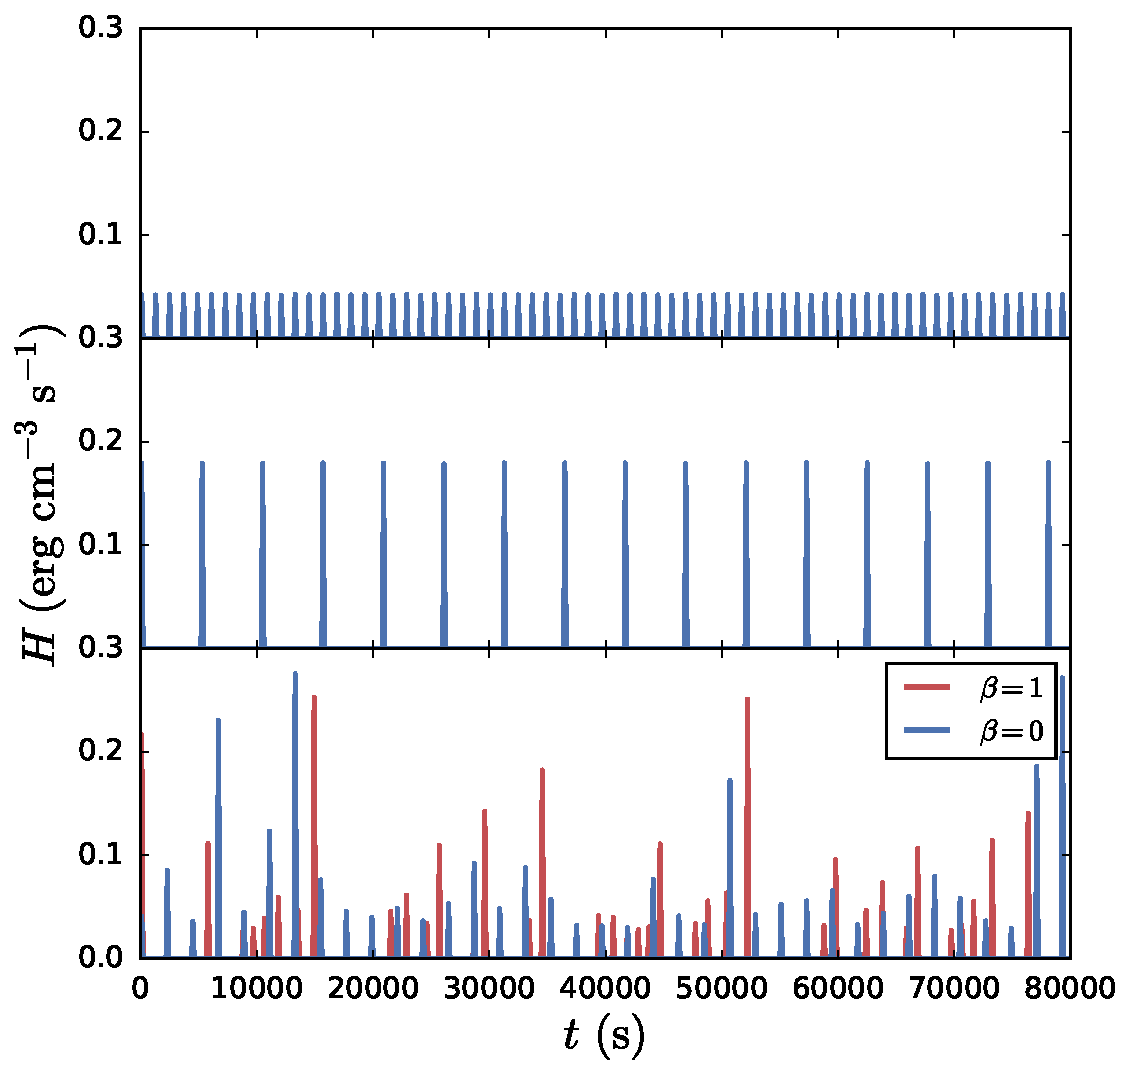
\includegraphics[width=\columnwidth]{figures/heating_functions.pdf}
		\caption{\textbf{Top}: uniform heating amplitudes for $t_N=1000$ s; \textbf{Middle:} uniform heating amplitudes for $t_N=5000$ s; \textbf{Bottom:} Heating amplitudes drawn from a power-law distribution with index $\alpha=-1.5$. The events shown in red have wait times that depend on the previous event energy while the events shown in blue have uniform wait times. The mean wait time in both cases is $\langle t_N\rangle=2000$ s.}
		\label{fig:heating_funcs}
	\end{figure}
%
	\par Recent observations have suggested that loops in AR cores are maintained at an equilibrium temperature of $T_{peak}\approx4$ MK \citep{warren_constraints_2011,warren_systematic_2012}. Using our modified two-fluid EBTEL model, we have estimated the corresponding time-averaged volumetric heating rate for a loop of half-length $L=40$ Mm to be  $H_{eq}\sim3.6\times10^{-3}$. In the single-fluid EBTEL model, this value is slightly lower because losses due to electron-ion collisions are ignored. Thus, to maintain an emission measure peaked about $T_{peak}$, for triangular pulses, the individual event heating rates are constrained by 
	\begin{equation}
		\label{eq:heating_rate_constraint}
		H_{eq} = \frac{1}{t_{total}}\sum_{i=1}^N\int_{t_i}^{t_i+\tau}\mathrm{d}t~Q(t) = \frac{\tau}{2t_{total}}\sum_{i=1}^NH_i,
	\end{equation}
	where $t_{total}$ is the total simulation time. Note that if $H_i=H_0$ for all $i$, the heating rate for each event is $H_i=H_0=2t_{total}H_{eq}/N\tau$. Thus, for $L=40$ Mm, $A=10^{14}$ cm$^2$, the average energy per event for a loop heated by $N=20$ nanoflares in $t_{total}=8\times10^4$ s is $\varepsilon=LAt_{total}H_{eq}/N\approx5.8\times10^{24}$ erg, consistent with the energy budget of the Parker nanoflare model. 
	%
	\par We define the heating frequency in terms of the waiting time, $t_N$, between successive heating events. Following \citet{cargill_active_2014}, the range of waiting times is $250\le t_N\le5000$ s in increments of 250 s, for a total of 20 different possible heating frequencies. Additionally, $t_N$ can be written as $t_N=(t_{total}-N\tau)/N$, where we fix $t_{total}=8\times10^4$ s and $\tau=200$ s. Note that because $t_{total}$ and $\tau$ are fixed, as $t_N$ increases, $N$ decreases. Correspondingly, $\varepsilon_i=LA\tau H_i/2$, the energy injected per event, increases according to \autoref{eq:heating_rate_constraint} such that the total energy injected per run is constant, independent of $t_N$.
	%
	\begin{figure}
		\centering
			\begin{tikzpicture}[node distance=2cm]
		%Draw the nodes
		\node (species) [ghost] {$\Sigma=\left\{
		\begin{array}{l}
			\mathrm{electron} \\
			\mathrm{ion} \\
			\mathrm{single}
		\end{array}
		\right.$};
		\node (ghost_ph) [ghost, below of=species] {};
		\node (alpha_pl) [ghost, left of=ghost_ph] {$\alpha=\left\{
		\begin{array}{l}
			-1.5 \\
			-2.0 \\
			-2.5
		\end{array}
		\right.$};
		\node (alpha_uni) [ghost, right of=ghost_ph] {uniform};
		\node (ghost_beta) [ghost, below of=alpha_pl]{};
		\node (beta_1) [ghost, right of=ghost_beta] {$\beta=1$};
		\node (beta_0) [ghost, left of=ghost_beta] {$\beta=0$};
		%Draw the arrows
		\draw [arrow] (species) -- (alpha_pl);
		\draw [arrow] (species) -- (alpha_uni);
		\draw [arrow] (alpha_pl) -- (beta_0);
		\draw [arrow] (alpha_pl) -- (beta_1);
		%\draw [arrow] (alpha_pl) -- (beta_2);	
	\end{tikzpicture}
		\caption{Total Parameter space covered. ``single'' indicates a single-fluid model. $\alpha$ is the power-law index and $\beta$ indicates the scaling in the relationship $Q\propto T_N^{\beta}$, where $\beta=0$ corresponds to the case where $t_N$ and the event energy are independent. Note that $(3~\alpha~\mathrm{values})\times(2~\beta~\mathrm{values})+\mathrm{uniform~heating}=$ 7 different types of heating functions.}
		\label{fig:parameter_space}
	\end{figure}
	%
	\par According to the nanoflare heating model of \citet{parker_nanoflares_1988}, turbulent loop footpoint motions twist and stress the field, leading to a buildup and subsequent release of energy. Following \citet{cargill_active_2014}, we let $\varepsilon_i\propto t_{N,i}^{\beta}$, where $\varepsilon_i,t_{N,i}$ are the total energy and waiting time following event $i$, respectively, and $\beta=1$ such that the event energy scales linearly with the waiting time. The reasoning for such an expression is as follows. Bursty, nanoflare heating is thought to arise from the stressing and subsequent relaxation of the coronal field. If a sufficient amount of energy is released into the loop, the field will need enough time to ``unravel'' and ``wind up'' again before the next event such that the subsequent waiting time is large. Conversely, if only a small amount of energy is released, the field will require a shorter unwinding time, resulting in a shorter interval between the subsequent events. Thus, this scaling provides a way to incorporate a more physically motivated heating function into a hydrodynamic model which cannot self-consistently determine the heat input based on the evolving magnetic field. \autoref{fig:heating_funcs} shows the various heating functions used for several example $t_N$ values.
	%
	\subsection{Heating Statistics}
	\label{subsec:heating_stats}
	%
	\par We compute the peak heating rate per event in two different ways: 1) the heating rate is uniform such that $H_i=H_0$ for all $i$ and 2) $H_i$ is chosen from a power-law distribution with index $\alpha$ where $\alpha=-1.5,-2.0,$ or $-2.5$. For the second case, it should be noted that, when $t_N\approx5000$ s, $N\sim16$ events, meaning the events from a single run do not accurately represent the distribution of index $\alpha$. Thus, a sufficiently large number of runs, $N_{R}$, are computed for each $t_N$ to ensure that the total number of events is $N_{tot}=N\times N_{R}\sim10^4$ such that the distribution is well-represented. \autoref{fig:parameter_space} shows the parameter space we will explore. For each set of parameters and waiting time $t_N$, we compute the resulting emission measure distribution for $N$ events in a period $t_{total}$. This procedure is repeated $N_R$ times until $N\times N_R\sim10^4$ is satisfied. Thus, when $t_N=5000$ s and $N\sim15$, $N_R=625$, meaning the model is run 625 times with a heating frequency of $t_N=5000$ s in order to properly fill out the event energy distribution.
	%
	\subsection{Non-equilibrium Ionization}
	\label{subsec:nei}
	%%
	\par When considering the role of nanoflares in the production of hot plasma in AR cores, it is important to take non-equilibrium ionization (NEI) into account \citep{bradshaw_explosive_2006,reale_nonequilibrium_2008}. In a steady heating scenario, the ionization state is an adequate measure of the electron plasma temperature. Because the heating timescale is long (effectively infinite), the ionization state has plenty of time to come into equilibrium with the electron temperature. 
	%
	\par In a nanoflare train, when the heating frequency is high, the loop is not allowed to drain or cool sufficiently between events, meaning the ionization state is kept at or near equilibrium. However, as the heating frequency decreases, the loop is allowed to cool and drain more and more during the inter-event period. If the heating occurs on a short enough timescale, the ionization state will not be able to reach equilibrium with the electron plasma before the loop undergoes rapid cooling by thermal conduction. Furthermore, if the frequency is sufficiently low so as to allow the loop to drain during the inter-event period, the ionization equilibrium timescale will increase. Thus, in the context of intermediate- to low-frequency nanoflares, NEI should be considered.
	%
	\par As in \citetalias{barnes_inference_2016}, we use the numerical code\footnote{This code has been made freely available by the author and can be downloaded at: \url{https://github.com/rice-solar-physics/IonPopSolver}.} outlined in \citet{bradshaw_numerical_2009} to asses the impact of NEI on our results. Given a temperature ($T(t)$) and density ($n(t)$) profile from EBTEL, we compute the non-equilibrium ionization states for Fe IX through XXVII and the corresponding effective electron temperature, $T_{eff}$ that would be inferred by assuming ionization equilibrium. Using $T_{eff}$, we are then able to compute a corresponding NEI emission measure distribution.
	%%
	\section{Results}
	\label{sec:results}
	%
	\par We now show the results of our loop simulations for each point in our multi-dimensional parameter space: species heated (single-fluid, electron or ion), power-law index ($\alpha$), heating frequency ($t_N$), and waiting-time/event energy relationship ($\beta$). In each 0D hydrodynamic simulation, a loop of half-length $L=40$ Mm is heated by $N$ triangular events of duration $\tau=200$ s and peak heating rate $H_i$ for a duration of $t_{total}=8\times10^4$ s. The average interval between subsequent events is $t_N$ (in the uniform and power-law case, $t_N,i=t_N$ exactly for all $i$). We focus primarily on the emission measure distribution, $\mathrm{EM}(T)$, and observables typically calculated from $\mathrm{EM}(T)$. In all cases, the coronal emission measure is calculated according to the method outlined in section 3 of \citetalias{barnes_inference_2016}. The corresponding NEI results, $\mathrm{EM}(T_{eff})$, are calculated similarly, but using $T_{eff}$ (see \autoref{subsec:nei}) instead of $T$. All results were processed using the IPython system for interactive scientific computing in Python \citep{perez_ipython:_2007} as well as the NumPy and Scipy numerical and scientific Python libraries \citep{van_der_walt_numpy_2011}. All results were visualized using the matplotlib graphics library \citep{hunter_matplotlib:_2007}.
	%%
	\subsection{Emission Measure Distributions}
	\label{subsec:em_dist}
	%
	\begin{figure*}[t]
		\centering
		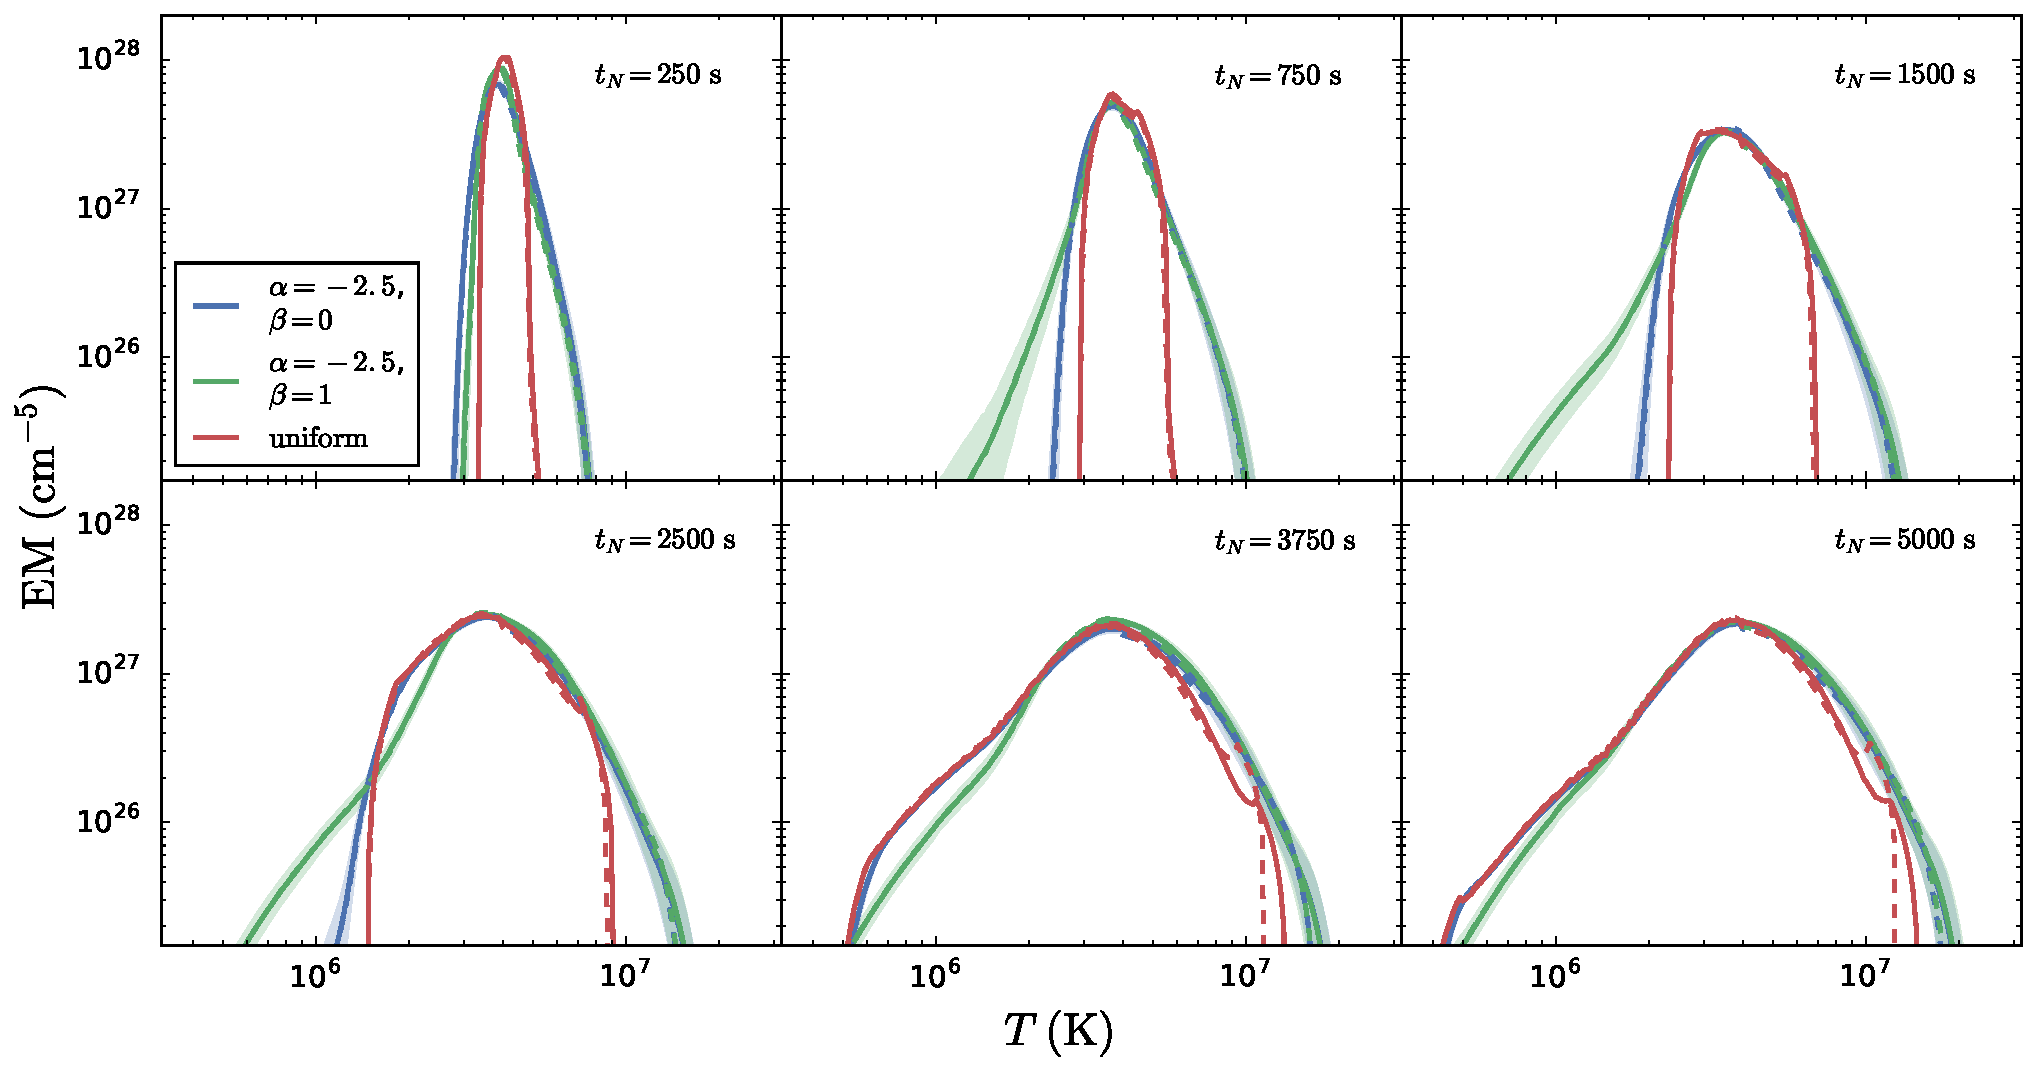
\includegraphics[width=2\columnwidth]{figures/em_grid_single_a25.pdf}
		\caption{Emission measure distributions for waiting-times $t_N=250,750,1500,2500,3750,5000$ s in the single-fluid case. The three types of heating functions shown are uniform heating rates (red), heating rates chosen from a power-law distribution of $\alpha=-2.5$ (blue), and heating rates chosen from a power-law distribution of $\alpha=-2.5$ where the time between successive events is proportional to the heating rate of the preceding event (green). The solid lines in the power-law cases show the mean $\mathrm{EM}(T)$ over $N_R$ runs and the shading indicates $1\sigma$ from the mean. The dashed lines denote the corresponding $\mathrm{EM}(T_{eff})$ distribution.}
		\label{fig:single_em}
	\end{figure*}
	%
	\begin{figure*}[t]
		\centering
		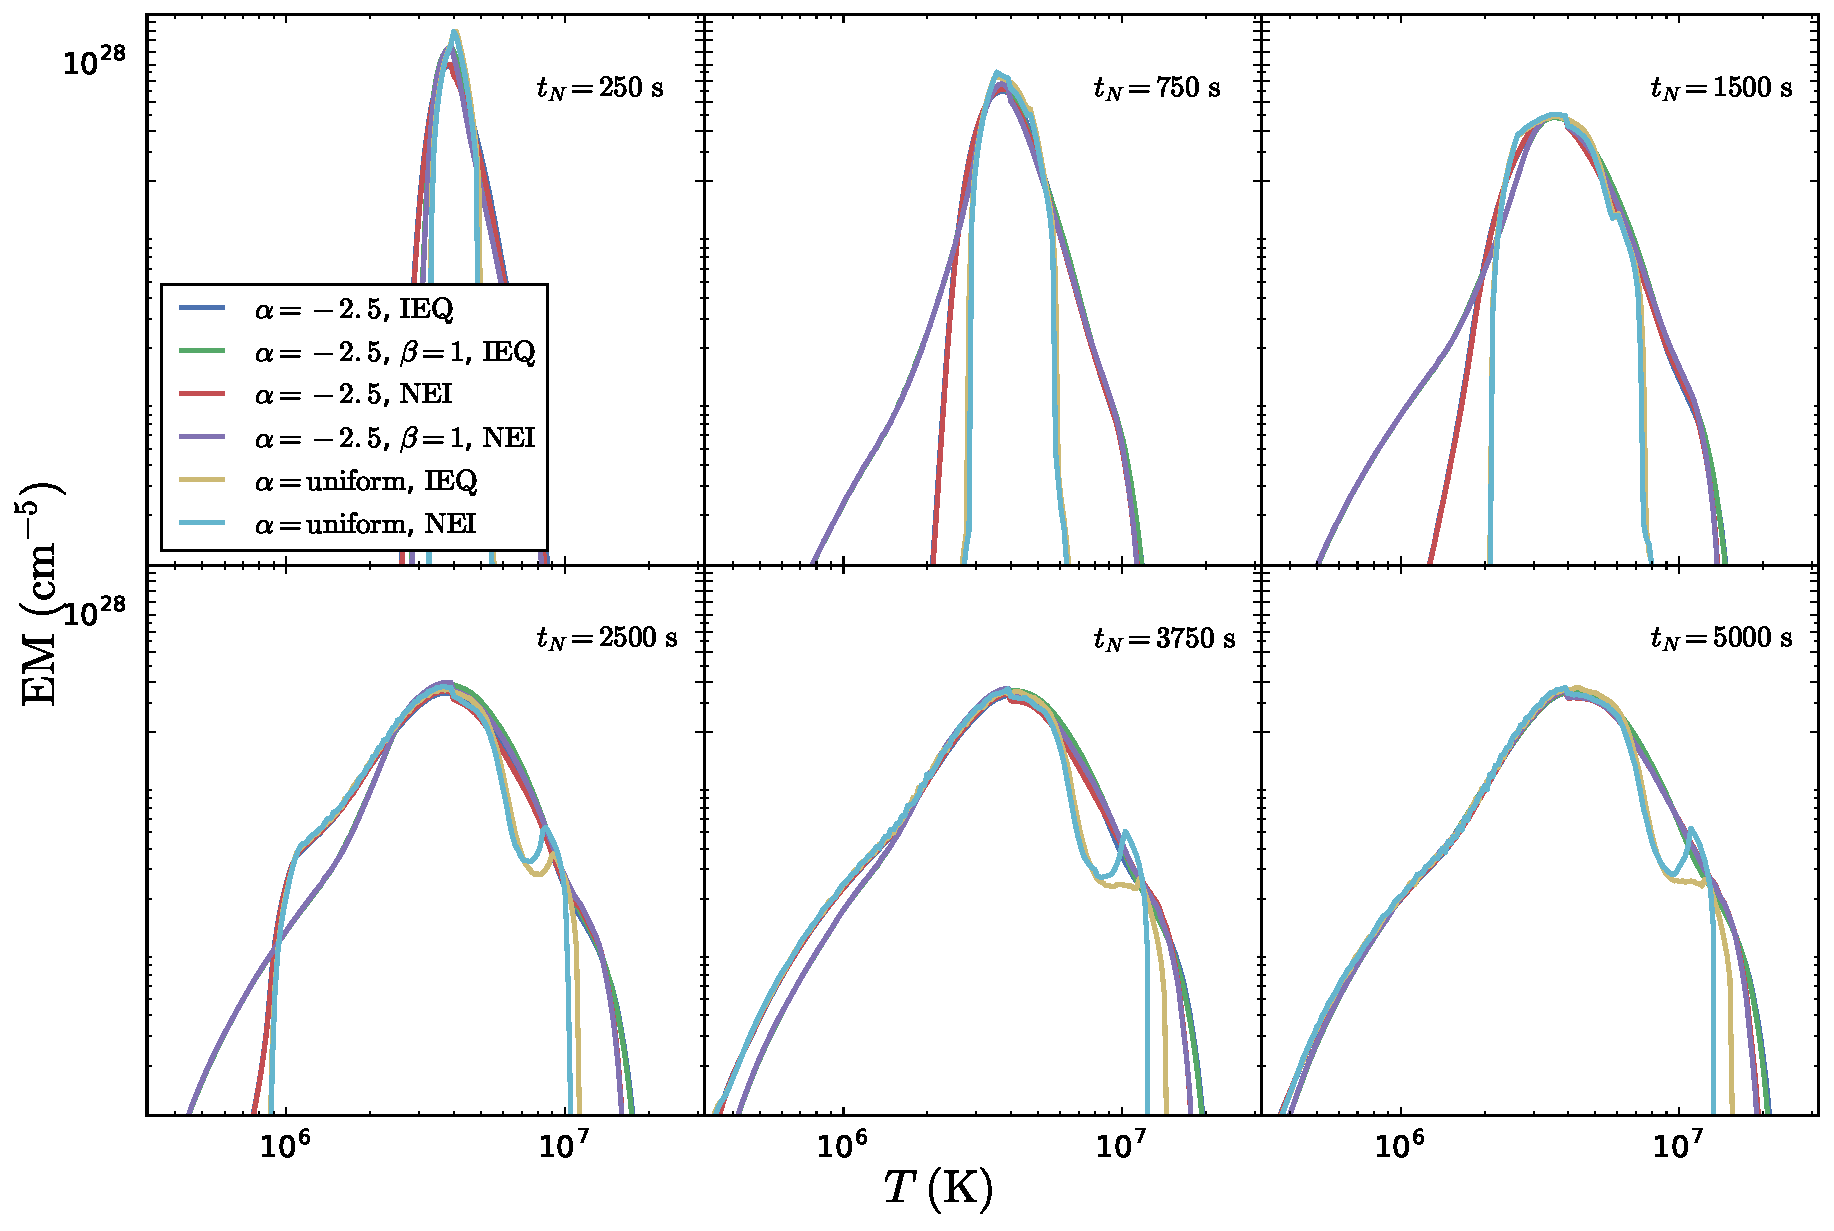
\includegraphics[width=2\columnwidth]{figures/em_grid_electron_a25.pdf}
		\caption{Same as \autoref{fig:single_em}, but for the case where only the electrons are heated.}
		\label{fig:el_em}
	\end{figure*}
	%
	\begin{figure*}
		\centering
		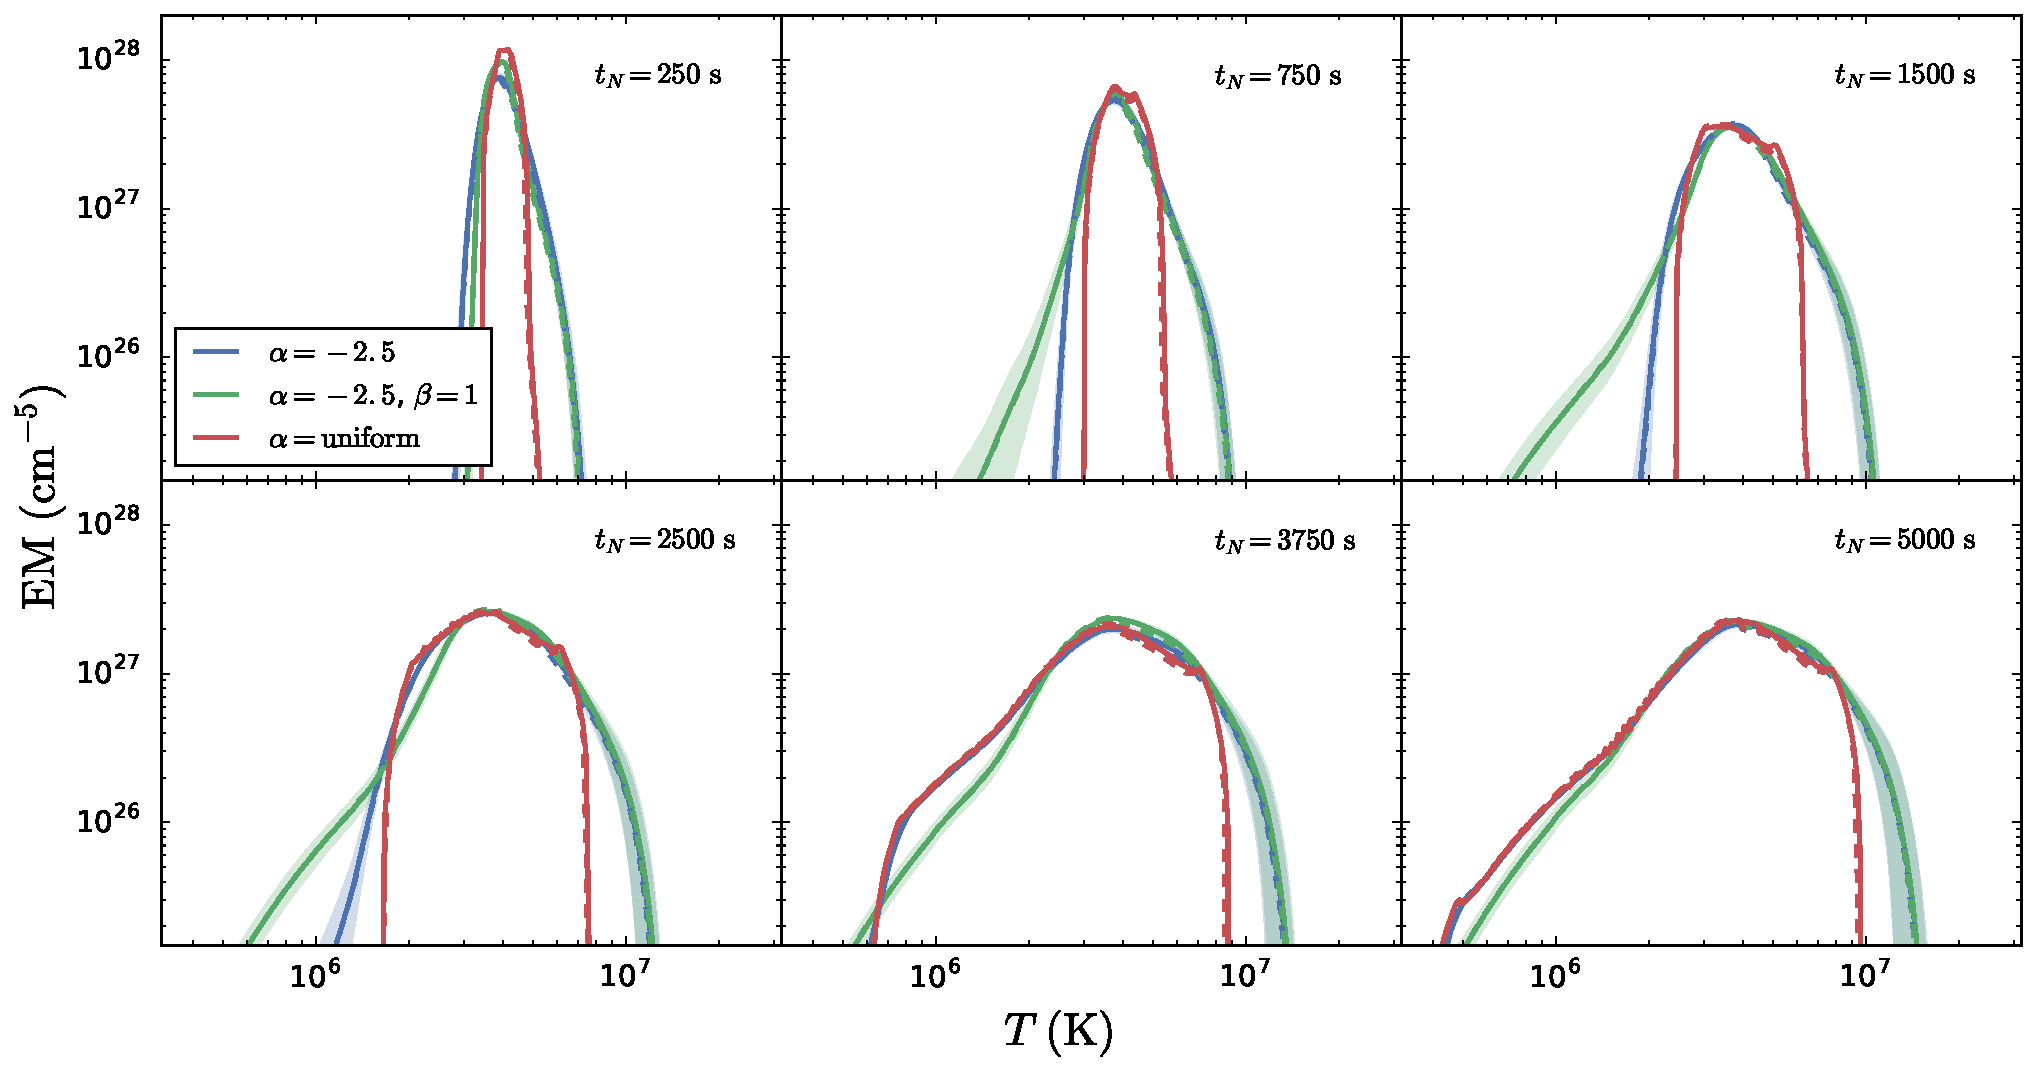
\includegraphics[width=2\columnwidth]{figures/em_grid_ion_a25.pdf}
		\caption{Same as \autoref{fig:single_em}, but for the case where only the ions are heated.}
		\label{fig:ion_em}
	\end{figure*}
	%
	\par In our first set of results, we compare $\mathrm{EM}(T)$ for three different types of heating functions, across six different heating frequencies. \autoref{fig:single_em}, \autoref{fig:el_em}, and \autoref{fig:ion_em} show the emission measure distributions in the single-fluid case, electron heating case, and ion heating case, respectively. Each panel in each figure corresponds to a different waiting time ($t_N$) and includes three different types of heating functions: uniform heating events (red), events chosen from a power-law distribution of index $\alpha=-2.5$ (blue), and events chosen from a power-law distribution of index $\alpha=-2.5$ where the time between successive events depends on the heating rate of the preceding event (green). Furthermore, the dashed lines denote the corresponding NEI cases, $\mathrm{EM}(T_{eff})$.
	%
	\par Recall from \autoref{subsec:heating_stats} that for those heating functions which choose peak heating rates from a power-law distribution, for each $t_N$, we run the model $N_R\sim(t_N+200)/8$ times. Thus, for each point in our parameter space, we produce $N_R$ $\mathrm{EM}(T)$ curves. In order to present our results compactly, the panels of \autoref{fig:single_em}, \autoref{fig:el_em}, and \autoref{fig:ion_em} each show the average over all $N_R$ curves. In this way, we account for the variations that may occur because of a lack/excess of strong heating events due to limited sampling from the distribution.
	%
	\par We look first at $\mathrm{EM}(T)$ for the single-fluid case, \autoref{fig:single_em}. Looking at all six panels, we note that as $t_N$ increases, $\mathrm{EM}(T)$ widens, extending to both cooler ($<4$ MK) and hotter ($>4$ MK) temperatures. $\mathrm{EM}(T)$ extends toward cooler temperatures because as $t_N$ increases and there is more time between successive heating events, the loop is allowed more time to cool both by radiation and enthalpy-driven cooling. $\mathrm{EM}(T)$ extends towards hotter temperatures for similar, but more subtle reasons. As $t_N\to0$, we approach the steady heating case in which conductive and radiative cooling exactly balance the heating. As $t_N$ increases and becomes comparable to and greater than a cooling time, the loop beceomes increasingly tenuous at the time of the subsequent heating event, allowing the loop to reach much hotter temperatures since radiative cooling is very inefficient at low densities and the heat flux saturates. In this way, $\mathrm{EM}(T)$ can ``see'' this greater range of temperatures, both hot and cool, provided it is allowed to undergo a typical heating and cooling cycle. The more curtailed this cycle is by continued reheatings, the more narrow $\mathrm{EM}(T)$ will be.
	%
	\par Looking at the different curves in each panel of \autoref{fig:single_em}, it is important to note that, although $\mathrm{EM}(T)$ for all three types of heating functions widen with increasing wait time, their dependence on $t_N$ is quite different. The uniform (red) and power-law (blue) $\mathrm{EM}(T)$ curves evolve similarly as they extend to cooler temperatures with increasing $t_N$ while the power-law, $\beta=1$ curve (green) extends to cooler temperatures much more rapidly. For example, at $t_N=1500$ s, both the uniform and power-law cases show little to no emission below 2 MK while the $\beta=1$ cases extends to temperatures well below 1 MK \citep{cargill_active_2014}. Contrastingly, on the hot side, the power-law and $\beta=1$ curves evolve nearly identically with increasing $t_N$ while the unfiorm heating case shows a cutoff at much lower temperatures, particularly for $t_N\le2500$ s. 
	%
	\par The $\mathrm{EM}(T)$ curves for the different types of heating functions shown in \autoref{fig:el_em}, in which only the electrons are heated, evolve similarly to those shown in \autoref{fig:single_em}. This is particularly true on the cool side where the density is sufficiently high, allowing the electrons and the ions to equilibrate such that there is no discernible difference compared to the single-fluid case. On the hot side, for $t_N\le750$ s, the electron and single-fluid cases are quite similar. However, for $t_N\ge1500$ s, $\mathrm{EM}(T)$ steepens just above 4 MK and then flattens out near 10 MK. This change in shape is most obvious in the uniform heating case where a distinct ``hot shoulder'' forms just above 10 MK. In the power-law cases, this feature is less pronounced and the $\mathrm{EM}(T)$ extends to slightly higher temperatures.
	%
	\par In \autoref{fig:ion_em} in which only the ions are heated, the cool side of the $\mathrm{EM}(T)$ is very similar to both the single-fluid and electron heating cases because the electron and ion populations are in equilibrium during this portion of the loop's evolution. On the hot side, for intermediate to low heating frequencies (i.e. $t_N\ge1500$ s), the $\mathrm{EM}(T)$ in the uniform heating case is truncated below 10 MK and in the power-law cases extends to just above 10 MK for the lowest heating frequency ($t_N=5000$ s). This cutoff at lower temperatures is due to the fact that electrons cannot ``see'' the ions until they have cooled well below their peak temperature. This is discussed in \citetalias{barnes_inference_2016} though in the single-pulse cases, the cutoff occured at lower temperatures. Additionally, in both the uniform and power-law cases, the peak of the $\mathrm{EM}(T)$ is wider for these low frequencies compared to those cases shown in \autoref{fig:single_em} and \autoref{fig:el_em}.
	%
	\par The dashed lines in the panels of \autoref{fig:single_em}, \autoref{fig:el_em}, and \autoref{fig:ion_em} show the corresponding $\mathrm{EM}(T_{eff})$ for each heating function type. Only the mean $\mathrm{EM}(T_{eff})$ over $N_R$ runs is shown for these results. In all three figures, for the intermediate to high frequencies (i.e. $t_N\le1500$ s), there is no discernible difference between $\mathrm{EM}(T)$ and $\mathrm{EM}(T_{eff})$. Furthermore, both of the power-law cases show little deviation from ionization equilibrium in the emission measure for even the lowest heating frequencies in the single-fluid, electron heating, and ion heating cases. For $t_N\ge2500$ s in the uniform heating case, in both \autoref{fig:single_em} and \autoref{fig:el_em}, $\mathrm{EM}(T_{eff})$ is truncated at slightly lower temperatures as compared to $\mathrm{EM}(T)$. This hot emission is relocated to cooler temperatures, resulting in a ``bump'' in the emission measure distribution near 10 MK. None of the panels of \autoref{fig:ion_em} show any significant difference between $\mathrm{EM}(T)$ and $\mathrm{EM}(T_{eff})$. This is because the electrons are essentially heated on a timescale dictated by the Coulomb collision frequency which is slow enough to ensure ionization equilibrium during the entire heating phase.
	%
	\subsection{Pre-nanoflare Density}
	\label{subsec:pre_nanoflare_density}
	%
	\begin{figure*}
		\centering
		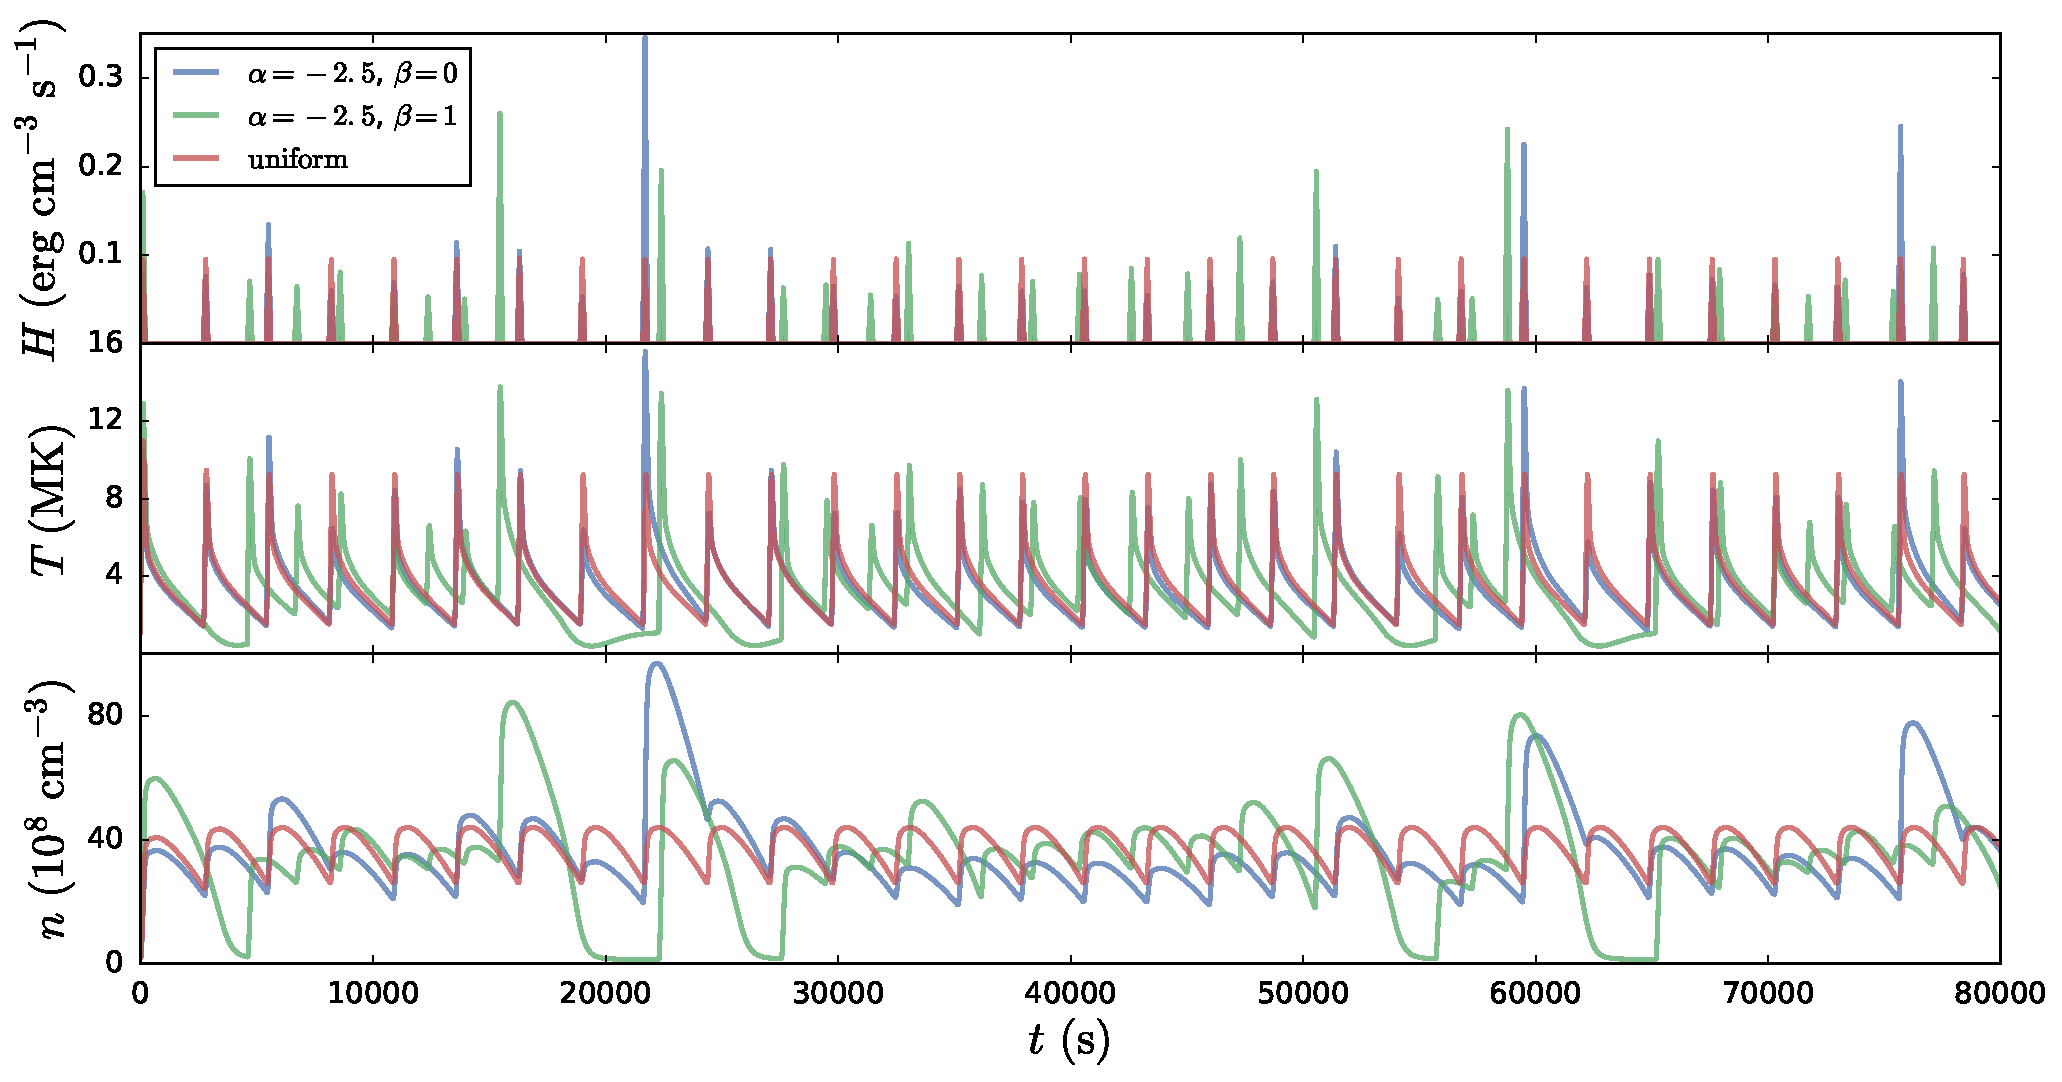
\includegraphics[width=2\columnwidth]{figures/nT_sample_curves_tn2500_electron.pdf}
		\caption{Example heating (top), temperature (middle), and density (bottom) profiles for the case in which only the electrons are heated and an intermediate heating frequency of $t_N=2500$ s. The three curves shown in each panel correspond to uniform heating rates (red), heating rates chosen from a power-law distribution of $\alpha=-2.5$ (blue), and heating rates chosen from a power-law distribution of $\alpha=-2.5$ where the time between successive events is proportional to the heating rate of the preceding event (green).}
		\label{fig:nT_sample_profiles}
	\end{figure*}
	%
	\par\hl{Mostly discussing differences between power-law and uniform on hot side and scaling/non-scaling on the cool side. Lead into this paragraph from the previous paragraph. Questions to answer: why do power-law cases extend to hotter temperatures for equivalent $t_N$? Why do power-law cases show little to no deviation from IEQ?}
	%
	\par In the single-fluid and electron heating cases, while $\mathrm{EM}(T)$ in the uniform and power-law heating cases generally agree for low-frequency heating ($t_N=5000$ s), for intermediate frequencies ($t_N\approx750-2500$ s), the power-law cases show an enhanced high-temperature component compared to the uniform case as seen in \autoref{fig:single_em} and \autoref{fig:el_em}.
	% 
	\par\autoref{fig:nT_sample_profiles} shows sample heating, temperature, and density profiles for an intermediate heating frequency ($t_N=2500$ s), in the case where only the electrons are heated, for the three different types of heating functions. In the uniform heating rate case (red), each event has a max heating rate of $H_0$ such that the loop undergoes $N\approx30$ identical heating and cooling cycles, each time reaching a maximum temperature and density of $T_{max,0}$ and $n_{max,0}$, respectively. Recall from \autoref{eq:heating_rate_constraint} that the total energy injected into the loop is constrained such that $H_0=(1/N)\sum_{i=1}^NH_i$. In the case where the heating rates are distributed according to a power-law, there will be many events where $H_i<H_0$ and a few events where $H_i\gg H_0$. 
	%
	\par The effect of these few higher energy events can be seen where the peak temperature of event $i$ is greater than $T_{max,0}$ in the two power-law cases (blue and green curves) in the middle panel of \autoref{fig:nT_sample_profiles} 
	%
	\subsection{Hot Plasma Diagnostics}
	\label{subsec:diagnostics}
	%%
	\par\hl{Discuss usefullness of hot slope versus cool slope via figure; discuss advantages of em ratio; discuss em ratio figures; break into subsections?}
	%%
	\begin{figure*}
		\centering
		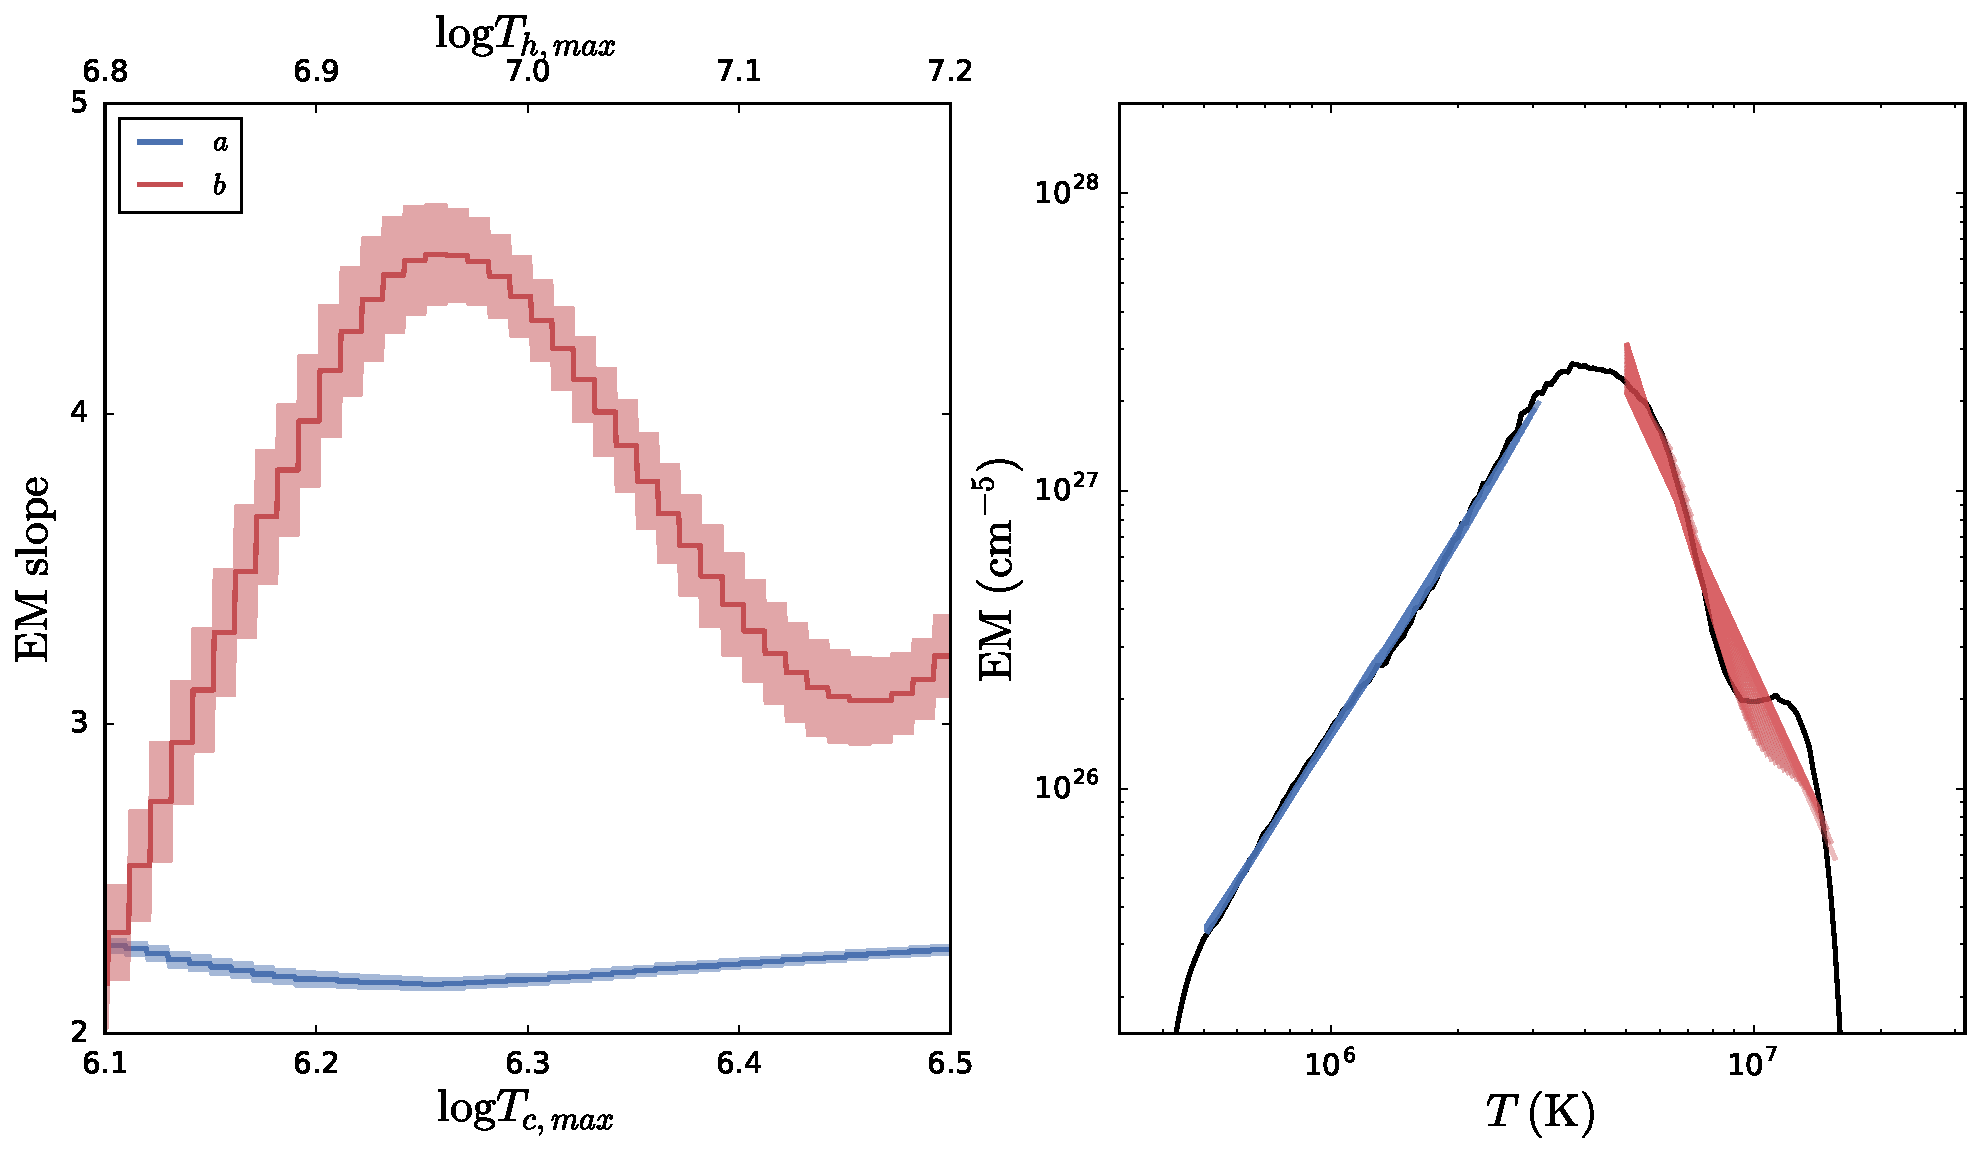
\includegraphics[width=2\columnwidth]{figures/em_slope_varying_bounds.pdf}
		\caption{Power-law fits to a sample emission measure distribution constructed from a loop plasma in which only the electrons were heated by events chosen from a power-law distribution with $\alpha=-2.5$ and equally spaced by an interval of $t_N=5000$ s. \textbf{Left:} $\mathrm{EM}(T)$ slope as a function of upper bound on fit interval for both the hot (red) and cool (blue) side of $\mathrm{EM}(T)$. The shading denotes the uncertainty of the fit. The bottom axis corresponds to the varying upper limit on the fit to the cool side while the top axis corresponds to the varying upper limit on the fit to the hot side. \textbf{Right:} $\mathrm{EM}(T)$ with the overlaid hot (red) and cool (blue) fit lines whose slopes correspond to those shown on the left. The cool power-law fits describe describe $\mathrm{EM}(T)$ for $T<4$ MK quite well while a similar fit on the hot side fails to accurately describe the shape of the emission measure distribution for $T>4$ MK.}
		\label{fig:em_slope_varying_bounds}
	\end{figure*}
	%%
	\begin{figure*}
		\centering
		\subfigure[]{%
		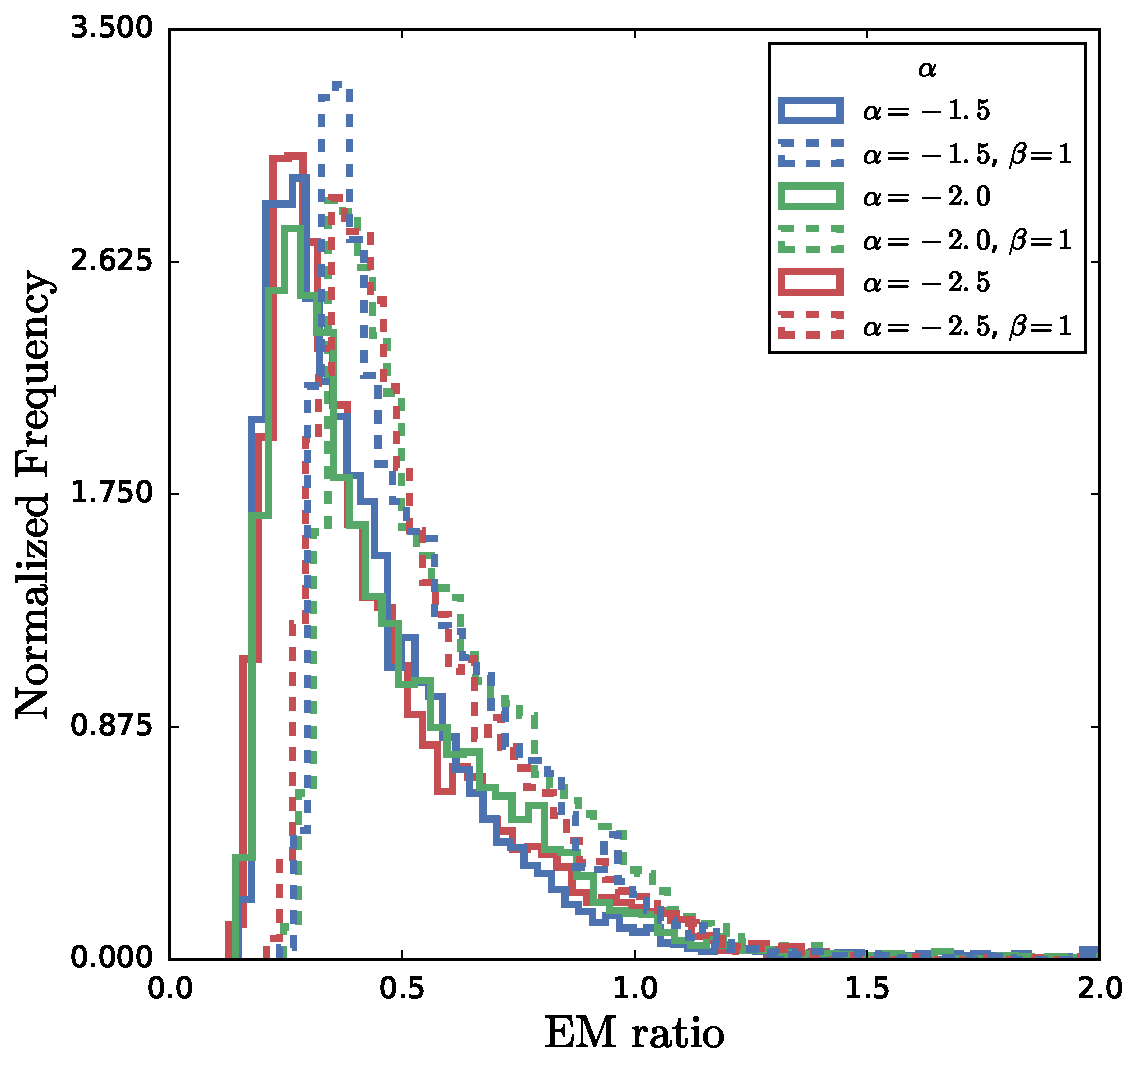
\includegraphics[width=\columnwidth]{figures/ratio_hist_alpha_electron_T2.pdf}
		}
		\subfigure[]{%
		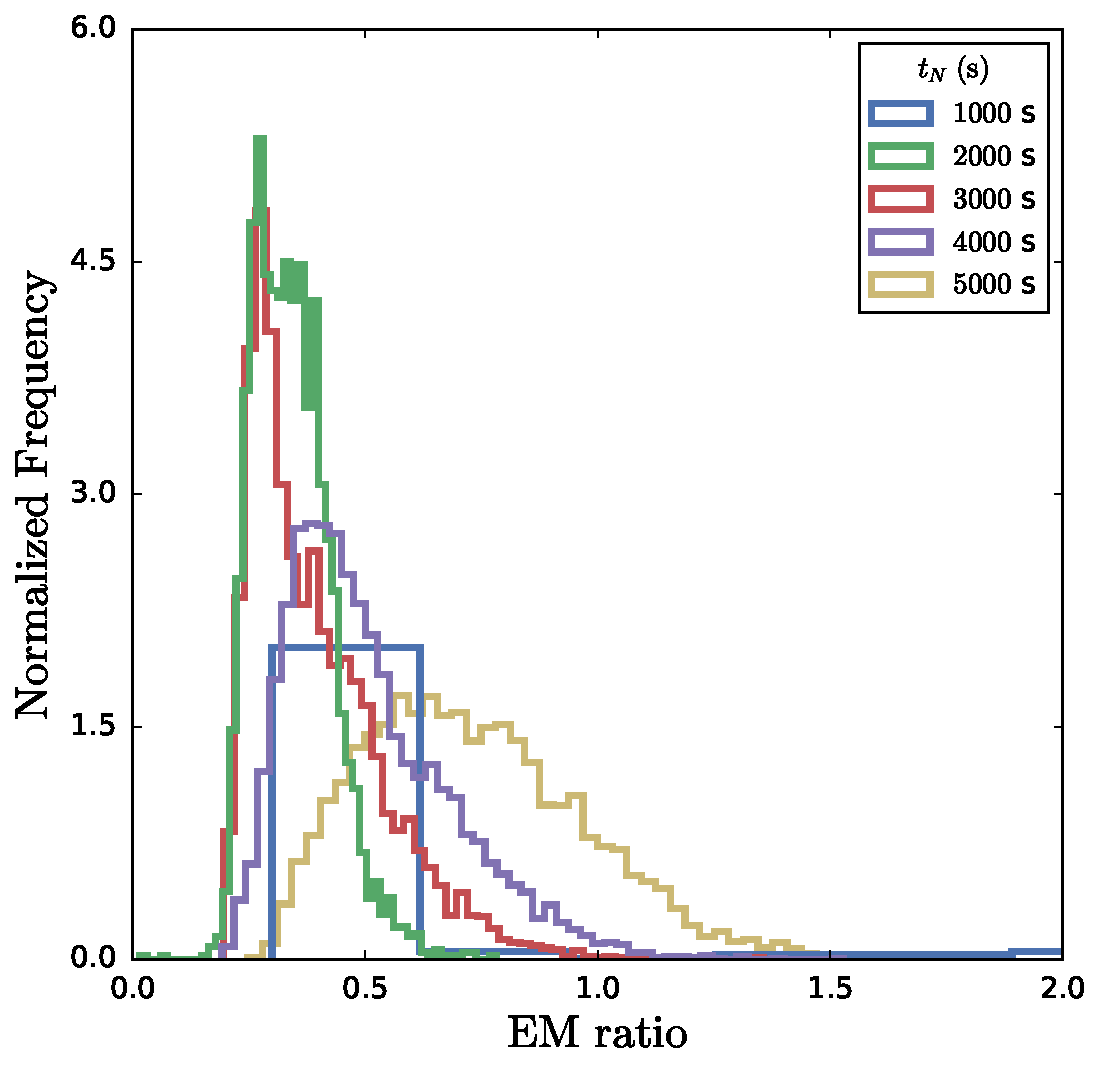
\includegraphics[width=\columnwidth]{figures/ratio_hist_twait_electron_T2.pdf}
		}
		\caption{Electron heating emission measure ratio for an EIS/MaGIXS line pair.\hl{Need a more descriptive caption here!}}
	\end{figure*}
	%%
	\begin{figure*}
		\centering
		\subfigure[]{%
		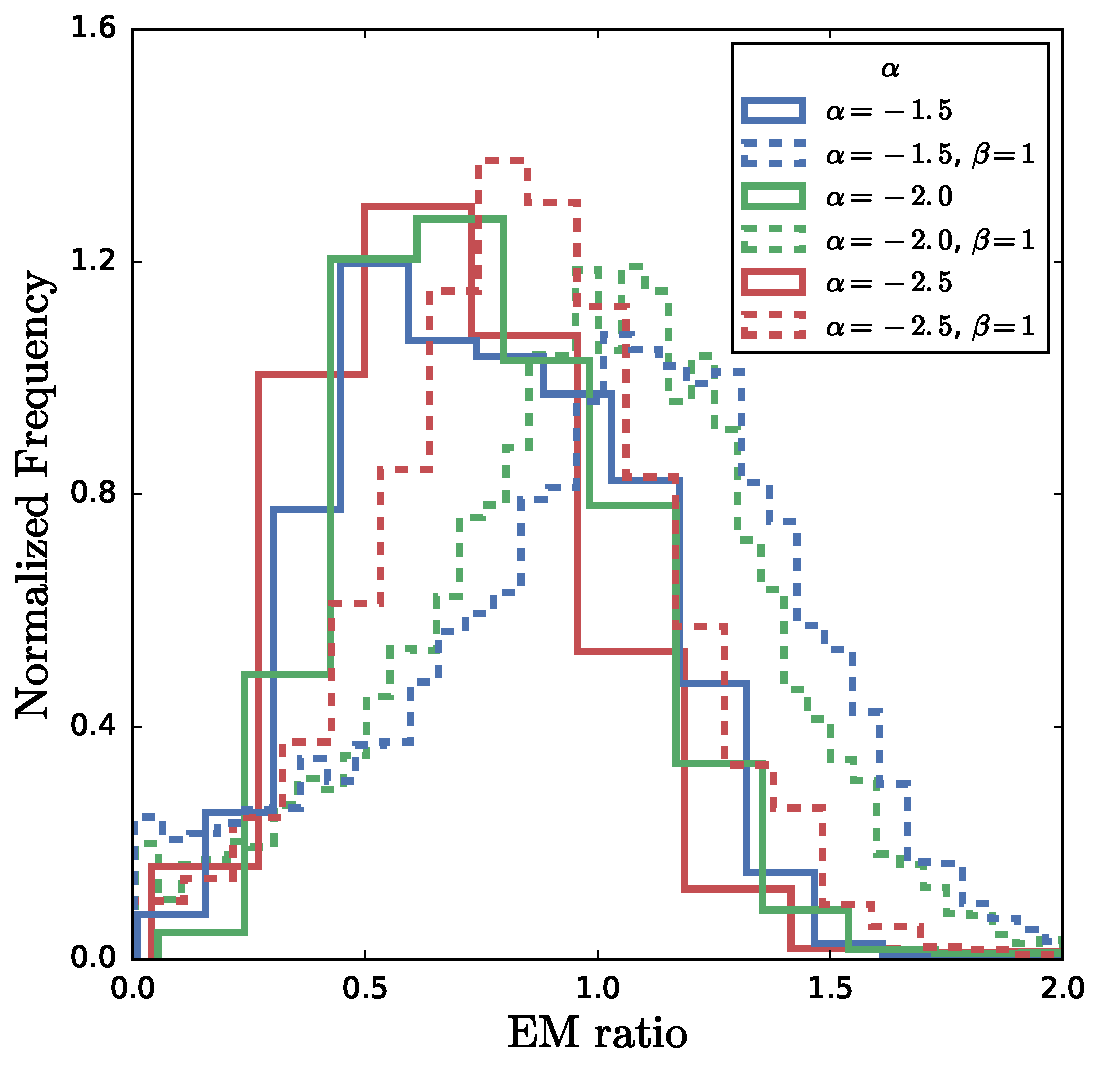
\includegraphics[width=\columnwidth]{figures/ratio_hist_alpha_ion_T2.pdf}
		}
		\subfigure[]{%
		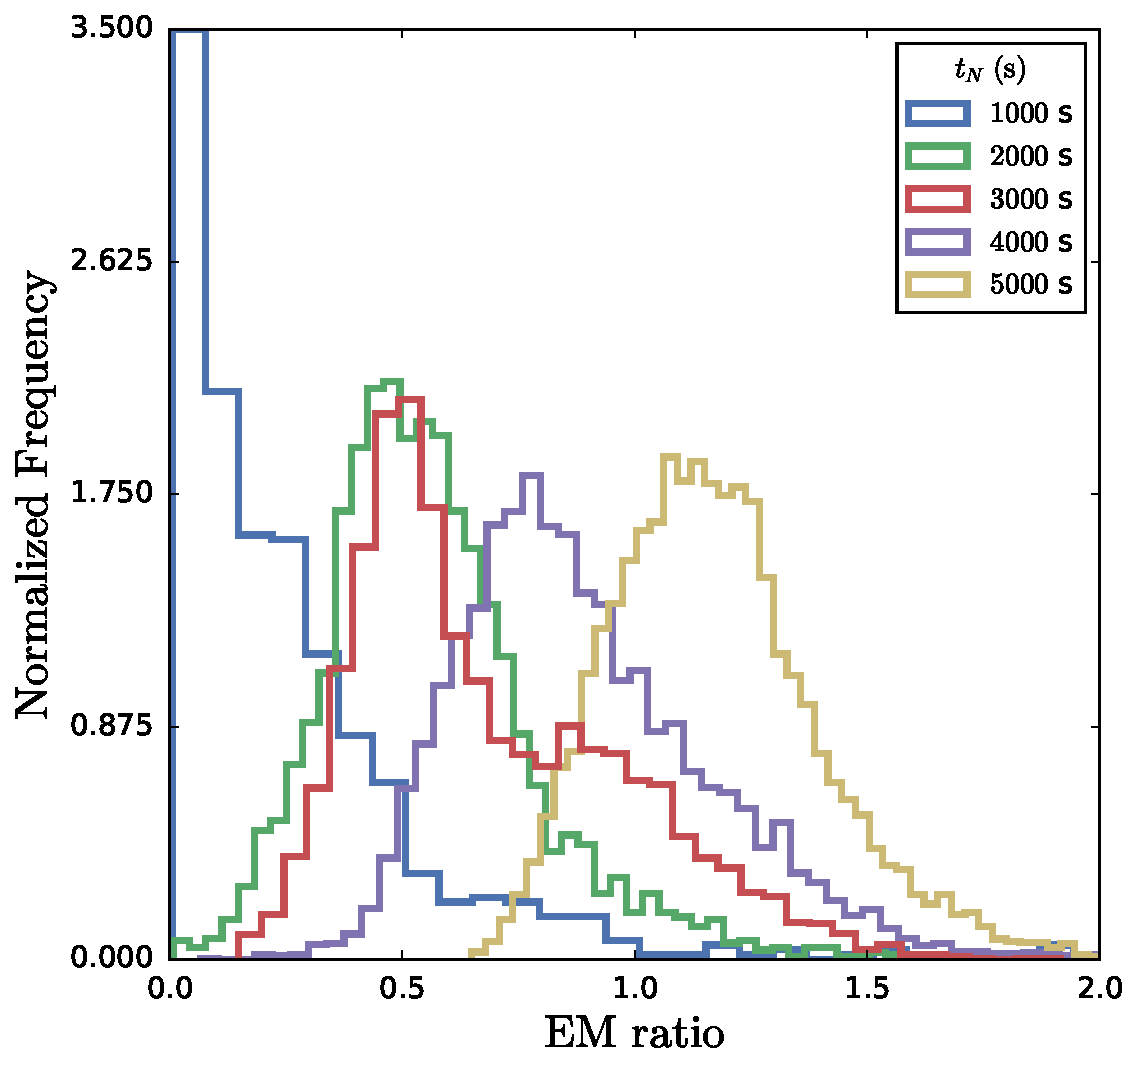
\includegraphics[width=\columnwidth]{figures/ratio_hist_twait_ion_T2.pdf}
		}
		\caption{Diagnostics figures}
	\end{figure*}
	%%
	%
	\par We now examine several observables often used to characterize the emission measure distribution. The most common observable is the emission measure slope $a$ such that $\mathrm{EM}\propto T^a$ for $10^{5.5}\le T\le10^{6.6}$ K. Both observational and modeling studies have found that $2<a<5$ \citep[see Table 3 of][]{bradshaw_diagnosing_2012} and in particular, \citet{cargill_active_2014} found that a heating function of the form $t_N\propto\varepsilon$ was needed in order to account for this range of slopes. Additionally, a similar scaling of $\mathrm{EM}\propto T^{-b}$ for $10^{6.6}\le T\le10^{7.0}$ has been claimed though measurements of $b$ have been subject to large uncertainties \citep{warren_systematic_2012}.
	%
	\par\autoref{fig:em_slope_varying_bounds} shows an example of how both $T^a$ and $T^{-b}$ can be fit to the cool and hot sides of $\mathrm{EM}(T)$, respectively. We fit $\log{\mathrm{EM}}$ to $a\log{T}$ on $\log{T_{c,min}}<\log{T}<\log{T_{c,max}}$ and $-b\log{T}$ on $\log{T_{h,min}}<\log{T}<\log{T_{h,max}}$ using the Levenburg-Marquardt algorithm for least-squares curve fitting as implemented in the SciPy scientific Python package \citep{van_der_walt_numpy_2011}. We fix the lower limit on each interval such that $T_{c,min}=10^{5.7}$ K and $T_{h,min} = 10^{6.7}$  K and vary the upper limits over $10^{6.1}<T_{c,max}<10^{6.5}$ and $10^{6.8}<T_{h,max}<10^{7.2}$. The left panel of \autoref{fig:em_slope_varying_bounds} shows the $a$ (blue) and $b$ (red) as a function upper limit of the fit interval, $T_{c,max}$ (bottom axis) and $T_{h,max}$ (top axis), respectively. The shading denotes the uncertainty of the fit. The right panel of \autoref{fig:em_slope_varying_bounds} shows the resulting fit lines superimposed on the emission measure distribution.
	%%%%%%%%%
	\par As seen in \autoref{fig:histos}, these histograms, denoted by type of slope (i.e. hot or cool) and species, are constructed in one of two ways: each distinct histogram (denoted by linestyle and/or color) is either representative of a distinct heating function (e.g. top row of \autoref{fig:histos}) or a distinct value of $t_N$ (e.g. bottom row of \autoref{fig:histos}). In the four panels of \autoref{fig:histos}, we choose to separate the cool emission measure slopes by type of heating function and the hot emission measure slopes by $t_N$. This means, for example, that the dot-dashed blue $\alpha=-1.5,\beta=1$ histogram in the upper left panel of \autoref{fig:histos} encapsulates cool emission measure slopes for $250\le T_N\le5000$ s while the solid blue $T_N=2000$ s histogram in the lower left panel includes emission measure slopes for all 10 types of heating functions (as listed in \autoref{fig:parameter_space} and the legend in the upper left panel of \autoref{fig:histos}). All histograms are normalized such that for each distribution $P(x)$, $\int_{-\infty}^{\infty}\mathrm{d}x~P(x)=1$. Additionally, the bin widths are calculated using the well-known Freedman-Diaconis formula \citep{freedman_histogram_1981}.
	%
	\section{Discussion}
	\label{sec:discussion}
	%
	\par The main points we emphasize from the results presented in \autoref{sec:results} are,
	\begin{enumerate}
		\item Cool emission measure slopes resulting from electron and ion heating are very similar and are well described by $\mathrm{EM}\propto T^a$. As noted in \citet{cargill_active_2014}, using the relation $Q\propto T_N^{\beta}$ yields $2\lesssim a\lesssim5$, consistent with observations.\label{itm:cool}
		\item Hot emission from electron heating results in an enhanced hot shoulder while the equivalent ion heating cases show a relatively flat peak and a steep dropoff near $10^7$ K. This effect is exacerbated as $t_N$ increases.\label{itm:hot}
		\item Hot emission due to both electron and ion heating is poorly described by the scaling $\mathrm{EM}\propto T^{-b}$. In the former, this is due to the flat hot shoulder between $10^7$ and $10^{7.5}$ K. In the latter case, the relatively flat peak and steep drop off near $10^7$ K do not allow for a power-law description of the hot emission.\label{itm:deriv}
		\item Using a power-law to describe the hot side of the $\mathrm{EM}$ distribution, single-fluid models predict less hot-emission than two-fluid models in which only the electrons are heated. In particular, for $T_N\ge4000$ s, our modified two-fluid EBTEL model predicts $3\le b\le3.5$ while the original single-fluid EBTEL model predicts $b\sim4.5$.\label{itm:histos}
		\item Including NEI does not impact the cool emission measure slope. In the case of electron heating and the single-fluid case, NEI enhances the mid-range hot $\mathrm{EM}$, but leads to a lower temperature cutoff. The emission measure distribution in the case of ion heating is unaffected. \label{itm:nei}
	\end{enumerate}
	%
	\par We first focus on \autoref{itm:cool}. In the range $6.0\le\log{T}\le6.6$, the loop is undergoing both radiative and enthalpy-driven cooling. During this phase, the density is high and the temperature low relative to the heating and conductive cooling phase. Looking at the fourth term on the right-hand side of \autoref{eq:press_e} and \autoref{eq:col_freq}, the coupling term between the two species is roughly $\propto\bar{n}^2(\bar{T}_e-\bar{T}_i)/\bar{T}_e^{3/2}$; as density increases, so does the coupling strength. While the loop is also draining in this temperature range, the density has already increased such that $\bar{T}_e\approx\bar{T}_i$ and until the next heating event, there is nothing to drive the two species out of equilibrium. Thus, because the two-species are evolving together in this regime, we expect their emission measure distributions to be the same.
	%
	\par In \autoref{itm:hot}, we see quite the opposite situation. In the heating and conductive cooling phases, the density is relatively low and the electron (or ion) temperature relatively high. Because the heating pulses we have used are relatively short (100 s), the heated species quickly reaches high temperatures and cools significantly by thermal conduction before Coulomb collisions can bring the two species back into equilibrium. Since the emission measure depends on the electron temperature, this means that in the event that only the electrons are heated, the emission  ``sees'' the full range of temperatures produced by heating and conductive cooling.
	%
	\par However, in the case of ion heating, in order for the emission measure to see the full range of temperatures resulting from the heating and conductive cooling by the ions, $\bar{T}_e=\bar{T}_i$ would have to hold for this entire phase. Instead, as the ions are impulsively heated, the electrons remain at a relatively low temperature, coupled only weakly to the ions because the loop has only just begun to fill. As the coronal density increases, the electrons come into equilibrium with the ions, but because thermal conduction is such an efficient cooling mechanism in the corona, the ions have now cooled far below the temperature to which they were initially heated. 
	\par The result is a severely truncated hot emission measure distribution as seen in \autoref{fig:ion_em}. Additionally, this effect is exacerbated at long $t_N$. For short $t_N$, the heating is essentially steady, meaning that the loop has little to no time to drain or cool between heating events. This keeps the density at a roughly constant, near-equilibrium value which inhibits rapid heating to high temperatures and keeps the electrons and ions in equilibrium. However, for longer $t_N$, the loop is allowed to drain significantly between each pulse. Thus, at the start of each heating event, the density is low, allowing the species to very quickly evolve out of equilibrium. 
	%
	\par Finally, \autoref{itm:nei} addresses the fact that NEI does not affect cool emission or emission due to ion heating, while it acts to enhance mid-range hot temperature emission and creates a lower-temperature cutoff in the single-fluid and electron heating cases as shown in \autoref{fig:teff_test_case}. As discussed in \citetalias{barnes_inference_2016} and \autoref{sec:intro}, if the heating occurs on a timescale faster than the ionization equilibration timescale, high temperatures will not be detectable because the charge states indicative of such temperatures will not have had time to form. Coolward emission is due to radiative and enthalpy-driven cooling and during this phase, the density is relatively high and the temperature is changing relatively slowly, meaning that ionization equilibrium can be assumed. 
	\par For hotward emission in the case of ion heating, we note that the effective heating timescale for the electrons is approximately $\tau_{ei}$, the coupling timescale. For $Q\approx10^{25}$ erg, the electron temperature increases relatively slowly (compared to the heating timescale of the ions) and only gets above several MK once the density has increased significantly. Thus, ionization equilibrium can be assumed because the electrons undergo no direct impulsive heating. In the cases of electron heating and the single-fluid case, the electrons undergo direct impulsive heating when the density is relatively low. This is what leads to the lower-temperature cutoff in $EM_{eff}$: at these high temperatures and low densities, the ionization equilibration timescale is significantly longer than the heating timescale and so these very high temperatures are never seen. 
	%
	\section{Conclusions}
	\label{sec:conclusions}
	%
	\par In this paper, we have used a modified two-fluid version of the popular EBTEL model to study the effect of preferentially heating the electrons or ions on the hot and cool emission measure slopes over a parameter space that includes the power-law index describing the distribution of event energies, $\alpha$, waiting time between successive heating events, $t_N$, and the scaling between the event energy and wait time, $\beta$. We have found that while there is little difference in the cool emission between the cases of electron and ion heating, the emission measure curves of the electron-heated loops have an enhanced hot shoulder due to faster loop filling times and steepened hot mid-range slope due to accelerated cooling by the Coulomb collisions while the ion-heated loops show a truncated emission measure distribution on the hot side. These differences become more prominent as $t_N$ increases. We note that given such a distinction in the $\mathrm{EM}$ distribution between the cases of electron and ion heating, the difference could be potentially observationally diagnosable by instruments such as MaGIXS, the Focusing Optics X-ray Solar Imager (FOXSI) \citep{krucker_focusing_2011}, or other future missions with adequate spectroscopic resolution in the hard X-rays.
	\par Furthermore, by comparing these results with emission measure distributions obtained from the original single-fluid EBTEL model, we have found that heating only the electrons and using a single power-law fit leads to significantly smaller hot emission measure slopes for equivalent values of $t_N$. Thus, using a single-fluid model to interpret observed hot emission measure distributions can potentially lead to a misdiagnosis of the heating frequency. Additionally, characterizing the hotward emission with a single power-law fit, as is common practice with cool emission, does not adequately capture all of the features of the hotward emission.
	%
	\par We note that in this study, we have constructed the most ideal emission measure curves by using the expression $\mathrm{EM}=n^2(2L)$; that is, we have not taken into account the many complications involved when computing emission measure distributions from observed spectral lines. For example, as we noted in \citetalias{barnes_inference_2016}, impulsive heating leads to NEI and a consequently lower effective temperature, meaning that the emission does not see the hottest temperatures during the conductive cooling phase. By computing test cases for electron heating, ion heating, and the single-fluid case, we have shown that NEI has the effect of steepening the hot emission measure distribution at very high temperatures and enhancing the mid-range hot temperature emission for the electron heating and single-fluid cases, but has no impact on the emission measure distribution in the case of ion heating. We stress that when interpreting observed hot emission in the context of simulation, two-fluid and non-equilibrium ionization effects should be properly taken into account in order to extract meaningful properties of the heating.
	%
	\section*{Acknowledgment}
	%
	WTB was provided travel support to the Coronal Loops Workshop VII held in Cambridge, UK, July 21-23, 2015, at which a preliminary version of this work was presented, by NSF award number 1536094. This work was supported in part by the Big-Data Private-Cloud Research Cyberinfrastructure MRI-award funded by NSF under grant CNS-1338099 and by Rice University.
	%
	%
	%Bibliography
	\bibliography{astrophys-abbrev.bib,references.bib}
	\bibliographystyle{apj}
	\clearpage
\end{document}